\documentclass{article}

\usepackage[version=3]{mhchem} % Package for chemical equation typesetting
\usepackage{siunitx} % Provides the \SI{}{} and \si{} command for typesetting SI units
\usepackage{graphicx} % Required for the inclusion of images
\usepackage{natbib} % Required to change bibliography style to APA
\usepackage{amsmath} % Required for some math elements 
\usepackage{epsfig}
\usepackage{subfigure}
\usepackage{epstopdf}
\usepackage{multirow}
\usepackage{ctex}
\usepackage{adjustbox}
\epstopdfsetup{outdir=./Figures/}
\graphicspath{{./Figures/}}
\setlength\parindent{0pt} % Removes all indentation from paragraphs

\renewcommand{\labelenumi}{\alph{enumi}.} % Make numbering in the enumerate environment by letter rather than number (e.g. section 6)

%\usepackage{times} % Uncomment to use the Times New Roman font

%----------------------------------------------------------------------------------------
%	DOCUMENT INFORMATION
%----------------------------------------------------------------------------------------

\title{计算机组成原理16位流水CPU实验报告
} % Title

\author{
小组编号 402\\
计24 田博 2012011346\\
计24 裘捷中 2012011345\\
计24 柯均洁 2012011335
} % Author name

\date{\today} % Date for the report

\begin{document}

\maketitle % Insert the title, author and date

\setcounter{tocdepth}{3} % Set the depth of the table of contents to show sections and subsections only

\tableofcontents % Print the table of contents

\section{实验成果综述}

实验使用了VHDL语言在FPGA上编程实现包含25条标准指令和5条扩展指令的16位类似MIPS指令集的CPU,支持多周期以及5级流水线。

为了解决结构冲突、数据冲突、控制冲突,使用了Forward Unit、Hazard Detection暂停流水等技术,提高流水线的效率。

扩展功能包括通过串口与PC机进行通信,从而运行监控程序,并在PC端控制CPU运行的指令(配合CPU运行的kernel程序)。其余功能还包括一个VGA显示,来同步显示当前的处理器状态,包括PC、寄存器、指令等,从而方便CPU的调试。

同时实验还开发了一系列Python脚本,用于自动生成entity表和管脚绑定信息,减少开发的工作量,避免粗心引起的错误,极大的提高了开发的效率。

项目可以通过https://github.com/dxmtb/CPU访问,提供了所有的源代码和测试程序,以及生成代码的脚本。bits文件夹包含了最终的CPU的bit文件,包含三个版本,cpu-12.5-final.bit是12.5MHz的CPU,cpu-click-final.bit是单步版本,cpu-vga.bit是单步并在VGA显示CPU状态的版本。

实验开发主要使用了XILINX ISE软件,开发版使用老师提供的THINPAD,包括FPGA、UART、RAM等部件。

\section{分工介绍} % (fold)
\label{sec:分工介绍}

\begin{itemize}
	\item 田博:CPU顶层结构(连线),控制器,阶段锁存器,VGA显示模块,RAM和串口模块,寄存器组;
	\item 裘捷中:数据通路和控制信号设计,Forward Unit,Hazard Detector,RAM和串口模块,ALU;
	\item 柯均洁:初版数据通路和控制信号,多路选择器,大部分实验报告。
\end{itemize}

% section 分工介绍 (end)

\section{关键设计介绍} % (fold)
\label{sec:关键设计介绍}

总体上来看,CPU分五级流水,就可以分为五个部分,下面结合实验中的一些困难详细介绍一些关键技术。

\subsection{访存与串口}
开发板为我们提供了两个RAM,其中RAM1与串口共享总线。我们的指令和数据都需要用到RAM,并且这种都要支持修改和读取操作。在最初的设计中,指令独占RAM2,而数据和串口共享RAM2,并且只实现了指令的读取操作,这样就避免了结构冲突。

之后发现监控程序需要修改指令内存,于是考虑到把指令和数据分开的动机已经消失,就把让串口独享RAM1的总线,从而简化串口的实现,而指令和数据都使用RAM2。这样就无法避免结构冲突,即如果需要写内存或者读取除当前指令以外的数据,都会与当前读取指令的操作冲突。我们的做法是暂停流水。具体是在Hazard Detection中检测MEM阶段有操作,并且这个操作不是针对串口,就暂停PC和锁存器。

另一个难点是,传统的实现中内存操作往往要多个周期,这会拖慢CPU的速度。我们采用“双边沿”的方法有效的在一个时钟周期内完成所有访存操作。其实并没有检测两个沿,具体时序是:

\begin{enumerate}
	\item 在上升沿,锁存器给出了MEM阶段的控制信号;
	\item 判断时钟为1时,就重置RAM信号,即置各个控制信号为1;
	\item 在时钟的下降沿,所有控制信号均已就绪,RAM信号已重置,可以根据当前操作给出新的控制信号;
	\item RAM的时钟较快,在控制时钟的下降沿不就,RAM的时钟上升沿,执行了MEM指令;
	\item 在时钟的上升沿,新的RAM数据(如果是读取的话)被送入锁存器,进入新的循环。
\end{enumerate}

\subsection{VGA扩展} % (fold)
VGA输出800x600的视频信号,通过对50MHz时钟进行分频来达到需要的工作频率。为了简化,我们仅仅使用两种颜色,黑色和白色。每一个16位的CPU状态,例如PC或者寄存器,每一个bit占一个40x40的一个方框,白色表示1,黑色表示0.

VGADisplayer向CoreDisplayer模块传输当前刷新的坐标,通过判断坐标的对应位置来判断显示哪个变量,并且判断当前位的值。

\subsection{代码自动生成}
代码自动生成包括生成entity表、portmap表、signal表、控制信号生成。

entity表比较简单,只要枚举每个VHDL文件,将相关关键字替换即可。

对于portmap,由于我们并不知道它的输入和输出是什么,所以比较棘手。我们可以观察到,每个portmap的输出必定是到一个signal,这样我们可以通过固定的明明规范,例如entity名下划线输出信号名来生成相应的signal,并绑定到那个signal。这样,我们只需要填充每个portmap的输入即可,并且通过名字就可以很容易判断signal的来源,大大减少了错误的可能。

对于控制信号,我们在代码开始对输出的variable赋值NULL语句的控制信号。每个控制信号和其取值有着规范的命名:控制信号的取值均为枚举类型,值为控制信号名下划线信号取值名。将控制信号表导出为csv,就方便了脚本进行分析和自动代码生成。

\section{实验结果}
\subsection{测试程序运行结果} 
CPU时钟:12.5M
执行时间(详细运行情况请见result1.MOV)
\begin{itemize}
    \item 测试程序1运行时间:12.029s
    \item 测试程序2运行时间:18.072s
    \item 测试程序3运行时间;14.015s
    \item 测试程序4运行时间:26.021s
    \item 测试程序5运行时间:14.021s
\end{itemize} 
\subsection{扩展指令运行结果}
程序的主要作用是往R0 load一个立即数,然后把R0的值放到R1,再比较R0和R1,如果两个相等,则往串口输出字母E
运行情况(详细运行情况请见result2.MOV)。

\begin{figure}[h]
\centering
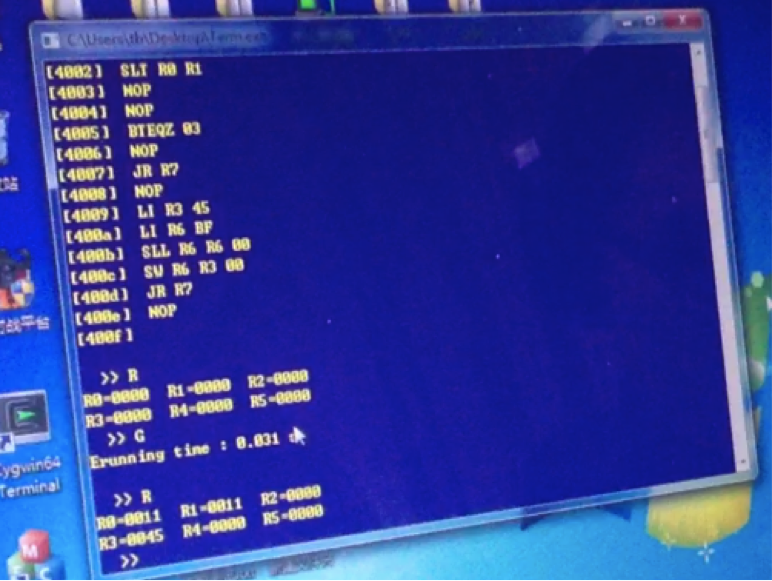
\includegraphics[width=1.1\columnwidth]{test.png}
\caption{扩展指令测试}
\label{fig:test}
\end{figure}

如图\ref{fig:test}所示,寄存器值发生了变化而且输出了字母E,因此程序成功运行

\subsection{VGA扩展运行结果}
\begin{figure}[h]
\centering
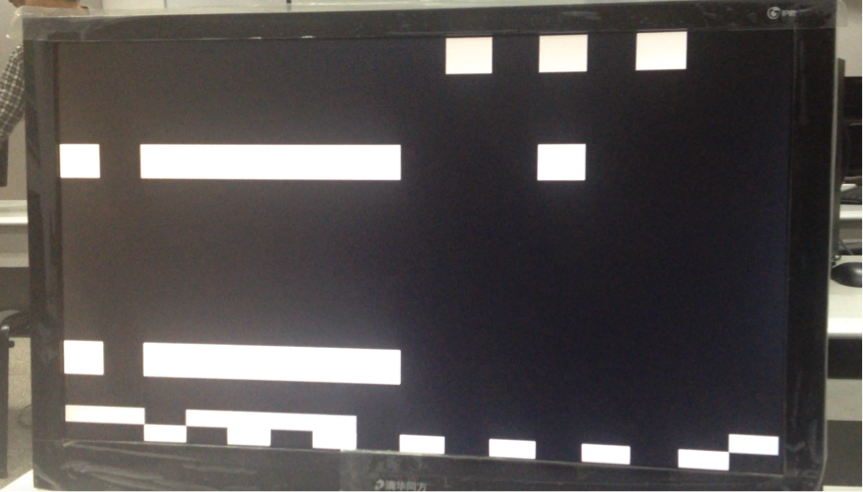
\includegraphics[width=1.1\columnwidth]{vga.png}
\caption{VGA扩展}
\label{fig:vga}
\end{figure}

我们用VGA模块在显示屏上显示寄存器信息
如图\ref{fig:vga}所示,从上到下依次为:PC、SP、IH、0-7号寄存器、当前运行指令的指令
通过按动按钮,我们可以观察到白块的移动,观察到寄存器值的变化,从而方便了程序的调试
详细运行情况请见result1.MOV

\section{实验总结}

通过这次实验,我们对CPU的各种细节有了更加充分的了解。更多的是,我们理解了团队合作的重要性:一个人做不到的事,有了其它人的帮助就可以做到。

我们由于数据同路的问题,直到DDL前一周的周五才开始编写代码,经过通宵和最后38小时的连续奋战,在检查当天的晚上8点终于完美运行所有功能,这与团队每个人的努力都分不开的。

实际上,我们最后一天想要尽快完成,在混乱不堪的内存串口模块中小修小补,直到前去检查也没有修补完成。到了检查现场,反而觉得超脱了急功近利的心情,静下心来对模块进行了重写,最后奇迹般的发现这个模块完美运行。这让我们体会到关键时刻保持清醒与镇定,摆脱急躁有多么重要。

这次大实验,所有的代码都是我们独立完成,尽管相对一些靠学长的组多花了许多时间,也少完成了一些扩展功能,但我们收获了人生的经验和感悟,这也是除了知识以外这个实验带给我们的最大收获。

\section{详细设计与实现}

\subsection{数据通路和控制信号设计图图}

见Figure~\ref{fig:datapath}~和Table~\ref{tb:control}。

\begin{figure}[h]
\centering
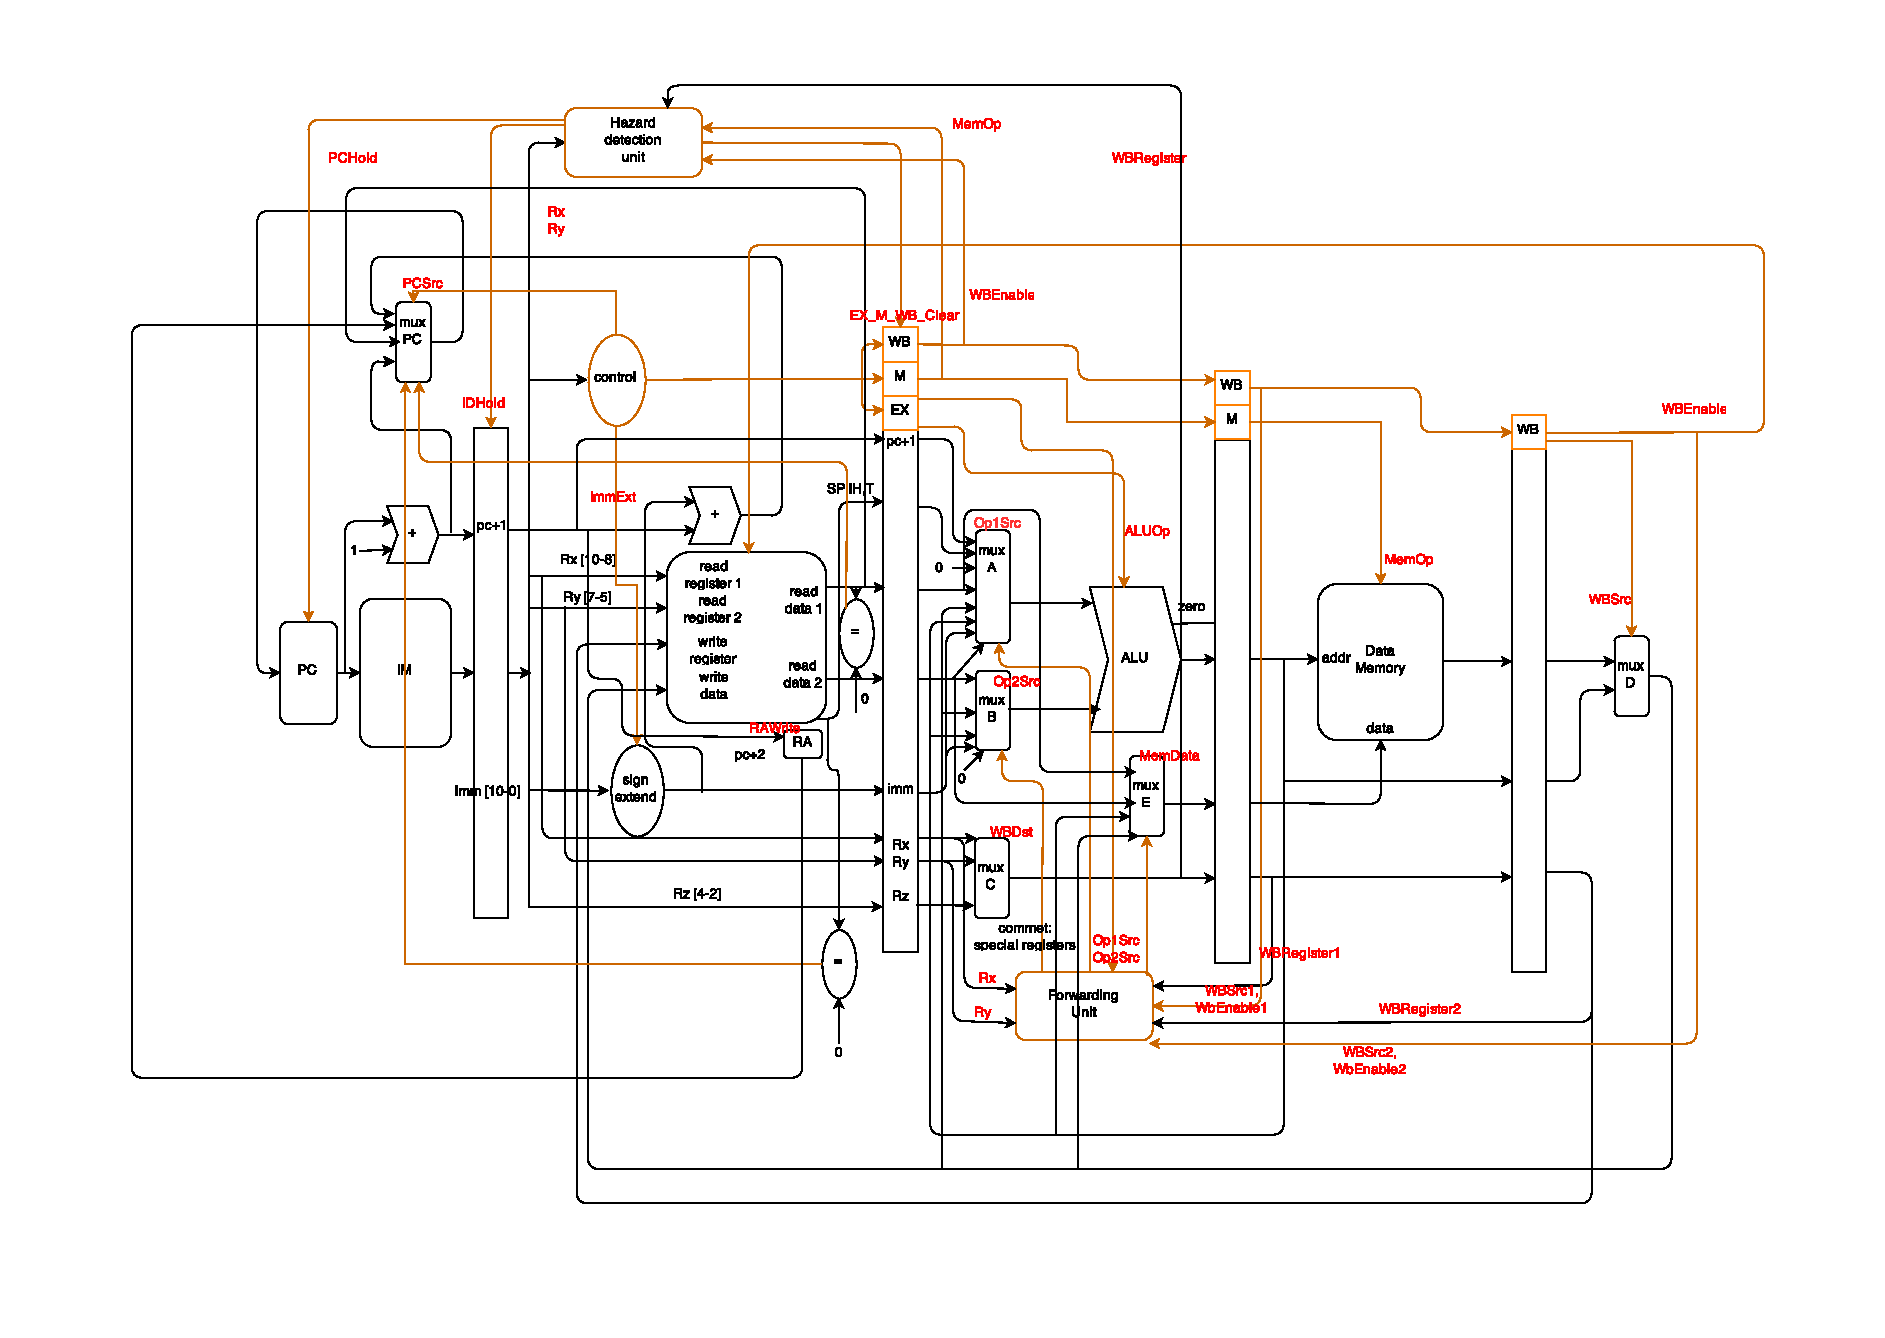
\includegraphics[width=1\columnwidth]{datapath.pdf}
\caption{数据通路和控制信号设计图}
\label{fig:datapath}
\end{figure}

\begin{table}
\caption{控制信号列表(*表示任意)}
\vspace{2mm}
\begin{adjustbox}{max width=\textwidth}
\label{tb:control}
\begin{tabular}[h]{c|c|c|c|c|c|c|c|c|c|c|c}
& PCSrc & ImmExt & RAWrite & Op1Src & Op2Src & WBDst & ALUOp & MemData & MemOp & WBSrc & WBEnable\\
NOP & PC+1 & * & No & * & * & * & * & * & No & * & If WBDst!= * then Yes\\
ADDIU &  & (Sign,7-0) &  & Rx & Imm & Rx & Plus &  &  & ALURes & \\
ADDIU3 &  & (Sign,3-0) &  & Rx & Imm & Ry & Plus &  &  & ALURes & \\
ADDSP &  & (Sign,7-0) &  & SP & Imm & SP & Plus &  &  & ALURes & \\
ADDU &  &  &  & Rx & Ry & Rz & Plus &  &  & ALURes & \\
AND &  &  &  & Rx & Ry & Rx & And &  &  & ALURes & \\
B & Branch-True & (Sign,10-0) &  &  &  &  &  &  &  &  & \\
BEQZ & Branch-Rx-0 & (Sign,7-0) &  &  &  &  &  &  &  &  & \\
BNEZ & Branch-Rx-1 & (Sign,7-0) &  &  &  &  &  &  &  &  & \\
BTEQZ & Branch-T-0 & (Sign,7-0) &  &  &  &  &  &  &  &  & \\
CMP &  &  &  & Rx & Ry & T & Sub &  &  & ALURes & \\
JR & Rx &  &  &  &  &  &  &  &  &  & \\
LI &  & (Zero,7-0) &  & Imm & 0 & Rx & Or &  &  & ALURes & \\
LW &  & (Sign,4-0) &  & Rx & Imm & Ry & Plus &  & Read & Mem & \\
LW\_SP &  & (Sign,7-0) &  & SP & Imm & Rx & Plus &  & Read & Mem & \\
MFIH &  &  &  & IH & 0 & Rx & Or &  &  & ALURes & \\
MFPC &  &  &  & PC+1 & 0 & Rx & Or &  &  & ALURes & \\
MTIH &  &  &  & Rx & 0 & IH & Or &  &  & ALURes & \\
MTSP &  &  &  & Rx & 0 & SP & Or &  &  & ALURes & \\
OR &  &  &  & Rx & Ry & Rx & Or &  &  & ALURes & \\
SLL &  & (Shift,4-2) &  & Ry & Imm & Rx & SLL &  &  & ALURes & \\
SRA &  & (Shift,4-2) &  & Ry & Imm & Rx & SRA &  &  & ALURes & \\
SUBU &  &  &  & Rx & Ry & Rz & Sub &  &  & ALURes & \\
SW &  & (Sign,4-0) &  & Rx & Imm &  & Plus & Ry & Write &  & \\
SW\_SP &  & (Sign,7-0) &  & SP & Imm &  & Plus & Rx & Write &  & \\
JRRA & RA &  &  &  &  &  &  &  &  &  & \\
JALR & Rx &  & Yes &  &  &  &  &  &  &  & \\
CMPI &  & (Sign,7-0) &  & Rx & Imm & T & Sub &  &  & ALURes & \\
MOVE &  &  &  & Ry & 0 & Rx & Or &  &  & ALURes & \\
SLT &  &  &  & Rx & Ry & T & If\_Less &  &  & ALURes & \\
\end{tabular}
\end{adjustbox}
\end{table}

\subsection{IF阶段}

\subsubsection{MUX\_PC}
\label{subsubsec:pc}
\paragraph{输入信号}
\begin{itemize}
\item PCSrc:控制MUX\_PC来选择下一个PC的取值,是顺序执行的PC+1或者是新的PC地址。取值情况为:
	\begin{itemize}
	\item PC1:等于PC+1,即顺序执行
	\item B:跳转到新地址Branch
	\item RA:跳转地址来自RA寄存器
	\item Rx:跳转地址来自Rx寄存器
	\item Rx\_0:R[x]=0时跳转到新地址Branch
	\item Rx\_1:R[x]!=0时跳转新地址Branch
	\item T\_0:T寄存器=0时跳转新地址Branch
	\end{itemize}
\item PCHold:
	\begin{itemize}
	\item PC是否保持,由Hazard Detect Unit控制。若PCHold为1,则保持原有的PC不变;若PCHold为0,则选择计算结果作为新的PC
	\end{itemize}
\end{itemize}
\paragraph{输出信号}
\begin{itemize}
\item Ret: 根据输入和控制信号输出相应的PC值
\end{itemize}

\subsubsection{RamHandler指令单元}

由于在我们的实现中,指令内存和数据内存使用的时同一块RAM(RAM2),所以对于RAM的操作我们统一用RamHandler这个entity来封装实现。
为保证说明时的一致性,我们会在\ref{subsec:mem}详细对这一模块进行描述。

\subsection{ID阶段}

\subsubsection{Controller控制单元}

\paragraph{单元描述}
\begin{itemize}
	\item 进行指令译码,产生之后阶段所需要的控制信号
	\item 默认初始化为NOP指令,即不写寄存器、不读内存 
\end{itemize}

\paragraph{输入信号}
\begin{itemize}
	\item INS: 16位指令 
\end{itemize}

\paragraph{输出信号}
\subparagraph{IFRegs}
IF阶段的控制信号,控制指令的跳转,由以下具体信号组成:
\begin{itemize}
	\item PCSrc : 选择哪个地址作为下一个PC,取值详见\ref{subsubsec:pc}
\end{itemize}
\subparagraph{IDRegs}
ID阶段的控制信号,由以下具体信号组成:
\begin{itemize}
	\item ImmExt:立即数扩展的形式
	\item RAWrite:是否要写RA寄存器
\end{itemize}
\subparagraph{EXRegs}
EX阶段的控制信号,由以下具体信号组成:
\begin{itemize}
	\item Op1Src: ALU操作数1的来源,MUX\_A选择信号
	\item Op2Src: ALU操作数2的来源,MUX\_B选择信号
	\item WBDst: 写回的目标寄存器。
	\item ALUOp:ALU的操作码。 
	\item MemData:读内存的地址来源寄存器
\end{itemize}
\subparagraph{MRegs}
MEM阶段的控制信号,由以下具体信号组成:
\begin{itemize}
	\item MemOp:内存的读取,取值为: 
		\begin{itemize}
			\item None:非访存操作
			\item Read:读取内存数据
			\item Write:写内存数据
		\end{itemize}
\end{itemize}

\subparagraph{WBRegs}
WB阶段的控制信号,由以下具体信号组成:
\begin{itemize}
	\item WBSrc:写回寄存器数据来源于ALU输出还是内存读取输出
	\item WBEnable:是否写回
\end{itemize}


\subsubsection{RegisterGroup寄存器组}

\paragraph{单元描述}

\subparagraph{维护寄存器组}
将编程可见的8个通用寄存器(编号0-7)以及T寄存器(编号8)、IH寄存器(编号9)、SP寄存器(编号10)封装到一起。RA寄存器单独存放。
\subparagraph{寄存器值的写入}
在一个CPU周期的上升沿写,写入的寄存器编号为write\_reg,由写回阶段的写回目的地信号WB\_Register\_out\_data.WBDst指定。
\subparagraph{寄存器值的读取}
读取的寄存器号由read\_reg1和read\_reg2指定。特殊寄存器由专门的输出信号regIH\_out、regSP\_out、regT\_out读出

\paragraph{输入信号}
\begin{itemize}
	\item clk:CPU时钟
	\item write\_enable:控制寄存器堆是否写入 
	\item read\_reg1、read\_reg2:要读取的两个寄存器编号
	\item write\_reg:要写入的寄存器编号 
	\item write\_data:要写入的值
\end{itemize}

\paragraph{输出信号}
\begin{itemize}
	\item reg1\_data、reg2\_data:读取的寄存器数据
	\item reg\_0\_out到reg7\_out、regIH\_out、regSP\_out、regT\_out:8个通用寄存器及Rsp、Rih寄存器的数据 
\end{itemize}

\subsubsection{RA寄存器}

\paragraph{单元描述}
由于RA寄存器用于特殊的JALR和JRRA指令,因此单独维护RA寄存器的读写。

\paragraph{输入信号}
\begin{itemize}
	\item clk:CPU时钟周期
	\item RAWrite:是否写RA寄存器 
	\item write\_data:用于写RA寄存器的数据,PC+1
\end{itemize}
\paragraph{输出信号}
\begin{itemize}
	\item RA:当前RA寄存器的值
\end{itemize}
\paragraph{实现细节}
由于写RA时只需要写入RPC,所以将输入的写数据write\_data取为PC+1,若需要写RA则将write\_data加1得到RPC写入RA寄存器

\subsubsection{SignExtend / ZeroExtend 符号/零扩展单元}

\paragraph{单元描述}

计算不同指令符号扩展或零扩展之后的16位立即数

\paragraph{输入信号}
\begin{itemize}
	\item imm\_in: 输入的需要扩展的立即数(11位)
	\item ImmExt: 由于不同指令存放立即数的长度和扩展类型是不同的,因此需要该控制信号标明立即数的位数及需要扩展的类型取值类型为
	\begin{itemize}
	\item ImmExt\_Sign\_7 立即数为7-0位,符号扩展
	\item ImmExt\_Sign\_3立即数为3-0位,符号扩展
	\item ImmExt\_Sign\_10立即数为10-0位,符号扩展
	\item ImmExt\_Sign\_4立即数为4-0位,符号扩展
	\item ImmExt\_Shift\_4\_2立即数为4-2位(相当于右移)
	\item ImmExt\_Zero\_7立即数为7-0位,零扩展
	\end{itemize}
\end{itemize}

\paragraph{输出信号}
\begin{itemize}
	\item imm\_out:16位扩展立即数
\end{itemize}

\subsubsection{Forwarding Unit 转发单元}

\paragraph{单元描述}

利用数据旁路技术来解决部分数据冒险

\paragraph{输入信号}
\begin{itemize}
	\item Rx, Ry
	\item Op1Src:ALU操作数来源,MUX\_A选择信号
	\item Op2Src:ALU操作数来源,MUX\_B选择信号
	\item wbsrc:当前指令要写回的结果来源于ALU的输出或访存结果 
	\item wbregister1:EX\_MEM阶段的那条指令写回的寄存器
	\item wbregister2:MEM\_WB阶段的那条指令写回的寄存器 
	\item wbenable1:EX\_MEM阶段的那条指令是否写寄存器	
	\item wbenable2:MEM\_WB阶段的那条指令是否写寄存器 
	\item memdata:写内存的数据来源
\end{itemize}
\paragraph{输出信号}
\begin{itemize}
	\item forwarda、forwardb、forwarde:MUX\_A、MUX\_B、MUX\_E是否使用forward数据及forward数据的来源,类型均为ForwardType,取值为:
	\begin{itemize}
		\item Forward\_None:不需要使用转发数据
		\item Forward\_From\_M\_WB:转发数据来自MEM\_WB阶段寄存器,也就是上一条指令的ALU计算结果
		\item Forward\_From\_WB:转发数据来自上一个MEM阶段得到的准备写回的数据,即访存所得数据
	\end{itemize}
\end{itemize}



\paragraph{实现细节}
\begin{itemize}
	\item 转发数据的来源有两个,一个是上一个阶段ALU的计算结果,另外一个是访存的结果。选择类型通过ForwardType的类型来指定
	\item 转发ALU计算结果的条件:
	\begin{itemize}
		\item 写回寄存器编号wbregister1与rx/ry/SP\_index/IH\_index相同
		
		\item 对应的写回使能wbenable1置1
		
		\item 当前指令写回的数据来源于ALU的计算结果
	\end{itemize}
	\item 转发访存结果的条件:
	\begin{itemize}
		\item 转发ALU计算结果的调节不满足
		\item 写回寄存器编号wbregister2与rx/ry/SP\_index/IH\_index相同
		\item 对应的写回使能wbenable2置1
	\end{itemize}
	\item 有些指令写回寄存器的值不是两个数操作后的运算结果,而是零扩展、某些寄存器值等等,可以将这种情况看做一个数和0相加,这样写回寄存器的值也可以看做ALURes来统一处理
\end{itemize}

\subsubsection{Hazard Detector 冒险测试单元}

\paragraph{单元描述}
\begin{itemize}
	\item 解决访存指令LW引起的数据冒险,若下一条指令Ex阶段需要使用LW指令的访存数据,则需要暂停流水,也就是插入NOP。
	
	\item 此外,由于指令和数据均存放在RAM2中,所以访问数据时也需要暂停流水 
\end{itemize}

\paragraph{输入信号}
\begin{itemize}
	\item wbenable:是否写回
	
	\item memop:ex阶段指令访存的操作,取/读/不操作 

	\item memop2:mem阶段指令访存的操作,取/读/不操作
	
	\item idrx、idry:id阶段的rx和ry 

	\item wbregister:写回的寄存器
	
	\item MemAddr:访问的内存地址 
\end{itemize}

\paragraph{输出信号}
\begin{itemize}
	\item exmwbclear:是否清空EX,MEM,WB阶段的信号
	
	\item Idhold:是否保持ID阶段指令 

	\item Pchold:是否保持PC
\end{itemize}

\paragraph{实现细节}

\subparagraph{LW引起的数据冒险暂停流水线作用条件}
	\begin{itemize}
	\item 需要写回寄存器,即wbenable置1
	\item memop==MemOp\_read,即这是一条LW指令
	\item idrx或idry与写回寄存器wbregister相等
	\end{itemize}

\subparagraph{MEM阶段访问RAM2暂停流水线作用条件}
由于我们把IM和DM都放在了RAM2上,所以一旦涉及到RAM2的读写操作,就无法正常读出下一条指令,因此必须暂定流水线一个周期。具体调节为:
	\begin{itemize}
		\item MEM阶段有读写RAM2操作
		\item 访存地址不是串口相关地址
	\end{itemize}


\subsection{EX阶段}

\subsubsection{ALU模块}

\paragraph{单元描述}

提供运算结果

\paragraph{输入信号}
\begin{itemize}
	\item Op1:ALU操作数1
	\item Op2:ALU操作数2 
	\item ALUOp:ALU的运算类型控制信号,取值为:
		\begin{itemize}
		\item ALUOp\_Plus:Op1 + Op2
		\item ALUOp\_And:Op1 and Op2
		\item ALUOp\_Sub:Op1 - Op2
		\item ALUOp\_Or:Op1 or Op2
		\item ALUOp\_SLL:Op1 逻辑左移Op2
		\item ALUOp\_SRA:Op1算术右移Op2
		\item ALUOp\_If\_Less:若Op1 < Op2则置为1,否则置为0
		\end{itemize}
\end{itemize}


\paragraph{输出信号}
\begin{itemize}
	\item ALURes:运算结果
\end{itemize}
	
\subsubsection{MUX\_A/MUX\_B:ALU操作选择器}
	
\paragraph{MUX\_A}
	
\subparagraph{单元描述}
选择数据作为ALU的第一个操作数

\subparagraph{输入信号}
	
\begin{itemize}
	\item 由EX阶段锁存器给出的的Op1src,指定操作数来源取值为
		\begin{itemize}
			\item Rx:R[x]
			\item Ry:R[y]
			\item SP:SP寄存器
			\item IH:IH寄存器
			\item Imm:16位立即数
			\item PC1:PC+1
		\end{itemize}
	\item 由Forward Unit产生的ForwardA,指定是否使用转发数据及转发数据来源。
	\item Rx, Ry SP, IH:分别表示相应寄存器的值
	\item Imm:立即数
	\item PC1:PC+1的值
	\item Data\_From\_WB:从WB阶段写回的数据
	\item Data\_From\_M\_WB:从MEM阶段写回的数据
\end{itemize}

\subparagraph{输出信号}
根据ForwardA的值以及控制信号Op1src选择对应的输入值作为该多路选择器的输出。
	
\paragraph{MUX\_B}
	
\subparagraph{单元描述}
选择数据作为ALU的第二个操作数
	
\subparagraph{输入信号}
\begin{itemize}
\item 由EX阶段锁存器给出的的Op2src,指定操作数来源,取值为
\begin{itemize}
\item Ry:R[y]
\item Imm:16位立即数
\item 0:零
\end{itemize}
\item Ry:R[y]
\item Imm:立即数
\item Data\_From\_WB:从WB阶段写回的数据
\item Data\_From\_M\_WB:从MEM阶段写回的数据
\item 由Forward Unit产生的ForwardB,指定是否使用转发数据及转发数据来源。
\end{itemize}
\subparagraph{输出信号}
根据ForwardB的值以及控制信号Op2src选择对应的输入值作为该多路选择器的输出。

\subsubsection{MUX\_C:写回寄存器编号选择器}	
\paragraph{单元描述}
选择写回寄存器的来源,由WBDst控制
\paragraph{输入信号}
\begin{itemize}
\item Rx, Ry, Rz
\item EX阶段锁存器给出的WBDst信号,取值为:
\begin{itemize}
\item Rx:写回rx字段的寄存器
\item Ry:写回ry字段的寄存器
\item Rz:写回rz字段的寄存器
\item SP:写回SP寄存器
\item IH:写回IH寄存器
\item T:写回T寄存器
\end{itemize}
\end{itemize}

\subparagraph{输出信号}
根据局WBDst选择对应的输入值作为该多路选择器的输出。

\subsubsection{MUX\_E:访存地址来源选择器}
\paragraph{单元描述}
选择访存地址的来源寄存器
\paragraph{输入信号}
\begin{itemize}
\item Rx, Ry
\item Data\_From\_WB:从WB阶段写回的数据
\item Data\_From\_M\_WB:从MEM阶段写回的数据
\item 由EX阶段锁存器给出的MemData信号,取值为:
\begin{itemize}
	\item Rx:来源于rx字段的寄存器
	\item Ry:来源于ry字段的寄存器
\end{itemize}
\item Forward Unit产生的ForwardE,指定是否使用转发数据及转发数据来源
\end{itemize}
\subparagraph{输出信号}
根据ForwardE的值以及控制信号MemData选择对应的输入值作为该多路选择器的输出。
	
		
\subsection{MEM阶段}
见关键设计介绍。

\subsection{WB阶段}
		
\subsubsection{MUX\_D:写回数据来源选择器}
		
\paragraph{单元描述}
选择访写回数据来源于ALU输出或者是访存结果
		
\paragraph{输入信号}
\begin{itemize}
\item WB阶段锁存器给出的WBSrc信号,取值为
		\begin{itemize}
			\item ALURes:写回数据来源于ALU的计算结果
			\item Mem:写回数据来源于访存读取的数据
		\end{itemize}
\item ALURes:来自ALU的计算结果
\item Mem:来自访存的结果
\end{itemize}
\paragraph{输出信号}
根据WBSrc信号选择对应的写回数据
		


\end{document}
